\chapter{Methods and Experiments}

\section{Single-Agent Bilateral Negotiation Environment (\gls{sbe})}
In this environment, agent represents the negotiator in negotiation mechanism.

\subsection{Independent Negotiator in NegMAS}
In the environment has just single learnable \gls{drl} negotiator. All of \gls{rl} algorithms can be tested in this specific environment. In the experiment of this thesis, \gls{dqn} and \gls{ppo} were tested in four learning scenarios:
\begin{itemize}
	\item single issue, acceptance strategy
	\item single issue, offer strategy
	\item multi-issues, acceptance strategy
	\item multi-issues, offer startegy
\end{itemize}

\subsection{Experiment}
MyDRLNegotiator vs AspirationNegotiator
\subsubsection{single issue}
Negotiation mechanism is \gls{saom}, split the learning strategy as two parts, acceptance strategy and offer strategy, 

Acceptance strategy: actions of agent are \texttt{Accept offer}, \texttt{Wait} and \texttt{Reject offer}. Observation of agent are offer of opponent and current time(running time, or current step of negotiation). Algorithms are \gls{dqn} (blue) and \gls{ppo} (red). Mean episode reward is shown in \ref{fig:acceptance-single-issue}

Offer strategy: Actions of negotiator are all outcomes set in mechanism. The observation is same as defined in the acceptance strategy. Before training the agent, normalize action and observation. Algorithm is DQN and PPO.

\begin{figure}[htbp]
\centering
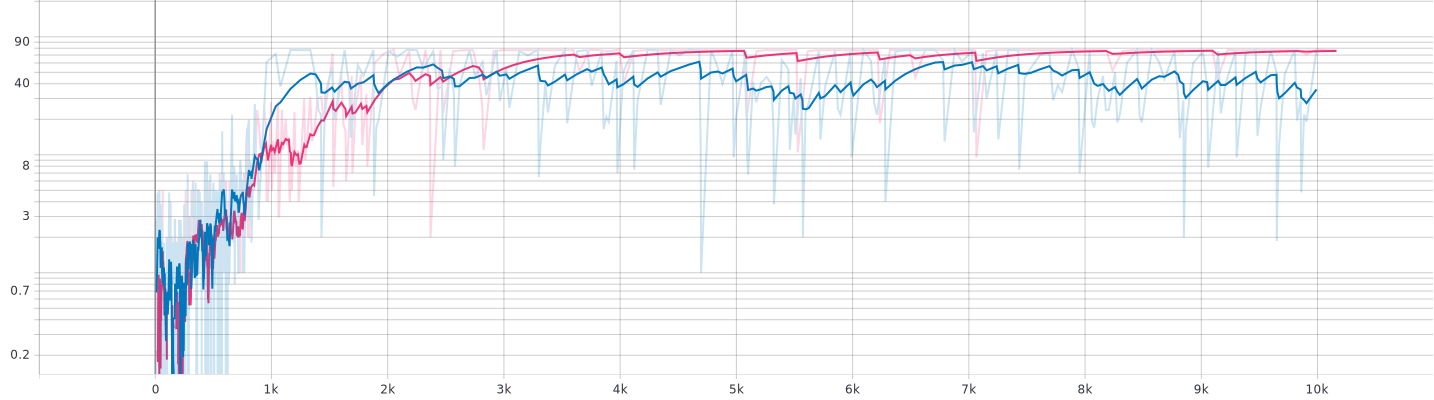
\includegraphics[width=0.80\textwidth]{./images/ac_s_dqn_ppo1_log_EpRe.png}
\caption{Episode mean reward of acceptance strategy under single issue}
\label{fig:acceptance-single-issue}
\end{figure}

\subsubsection{multi issues}

\subsection{Evaluation}

\section{Multi-Agent Concurrent Bilateral Negotiation Environment (\gls{mcbe})}
In this environment, agent represents the factory manager and negotiation controller in standard \gls{scml} and \gls{scml} OneShot, respectively.

The environment provides all informations that are needed for reinforcement learning. Action, Observation and Reward are passed through callback functions defined in the class \texttt{Scenario}. In addition, class \texttt{Scenario} contains predefined informations, such as structure of supply chain network, parameters of learnable agents and so on.

\gls{mcbe} is shown as in.

\subsection{\gls{maddpg} in \gls{scml}}
Shown in \ref{fig:method-maddpg-scml}

\begin{figure}[htbp]
\centering
\includegraphics[width=0.80\textwidth]{./images/scml-maddpg.png}
\caption{maddpg used in multi agents concurrent negotiation based on standard \gls{scml}}
\label{fig:method-maddpg-scml}
\end{figure}

Actors output actions as inputs to related agents interacting with the environment. Agents interacting with environment outputs the observation and reward as the inputs to related agents trained in the model. 

The same agent interacting with environment may be have many related trainable agents as the part of agent(e.g. one seller, one buyer) in the model. The detail of interactive logic is shown below in \ref{fig:interacting-logic-maddpg-scml}

\begin{figure}[htbp]
\centering
\includegraphics[width=0.90\textwidth]{./images/scnk.png}
\caption{Interactive logic based on the perspective of \gls{scml}}
\label{fig:interacting-logic-maddpg-scml}
\end{figure}

\begin{algorithm}[H]
  \SetAlgoLined
  \KwData{this text}
  \KwResult{how to write algorithm with \LaTeX2e }

  initialization\;
  \While{not at end of this document}{
    read current\;
    \eIf{understand}{
      go to next section\;
      current section becomes this one\;
      }{
      go back to the beginning of current section\;
      }
    }
  \caption{How to write algorithms}
\end{algorithm}

\subsection{\gls{qmix} in \gls{scml}}
test
\subsection{Experiment}
\subsubsection{Concurrent Neogtiations in standard \gls{scml}}
\subsubsection{Concurrent Negotiations in OneShot \gls{scml}}
\textbf{self-play}

Episode mean reward curve is shown in \ref{fig:oneshot-self-play}

\begin{figure}[htbp]
\centering
\includegraphics[width=0.80\textwidth]{./images/oneshot_self_play.png}
\caption{Episode mean reward of self paly under SCML OneShot}
\label{fig:oneshot-self-play}
\end{figure}

\textbf{play with other agent}

My agent vs GreedyOneShotAgent

Episode mean reward curve is shown in \ref{fig:oneshot-my-vs-greedy}

\begin{figure}[htbp]
\centering
\includegraphics[width=0.80\textwidth]{./images/oneshot_my_vs_greedy.png}
\caption{Episode mean reward of my agent vs GreedyOneShotAgent under SCML OneShot}
\label{fig:oneshot-my-vs-greedy}
\end{figure}

\subsection{Evaluation}

\section{Conclusion}